\documentclass{beamer}
\usepackage[utf8]{inputenc} 
\usepackage{times}
\usepackage[T1]{fontenc}
\usepackage[spanish]{babel}
\usepackage{graphicx}
\usepackage[hidelinks]{hyperref}
\usepackage{color}
\graphicspath{{images/}}
\title{Análisis de los precios de algunos productos en Habana del Este.}
\date{Facultad de Mátematica y Computación}
\author{Jennifer de la Caridad Sánchez Santana}
\usetheme{PaloAlto}
\usecolortheme{default}
\setbeamercovered{transparent}


\begin{document}
\begin{frame}
\titlepage
\end{frame}

\begin{frame}{Cerveza}
    
    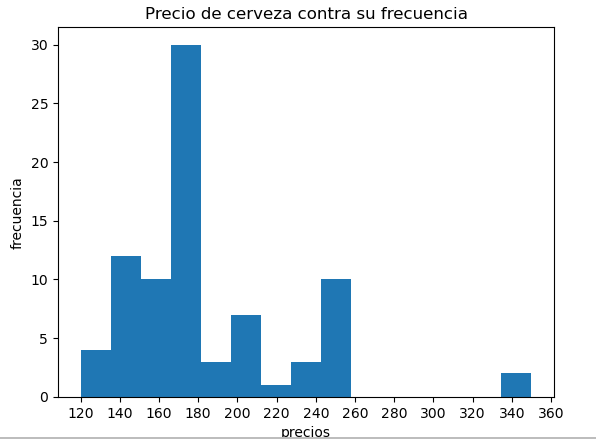
\includegraphics[scale=0.5]{precio cerveza.png}
    \end{frame}

\begin{frame}
    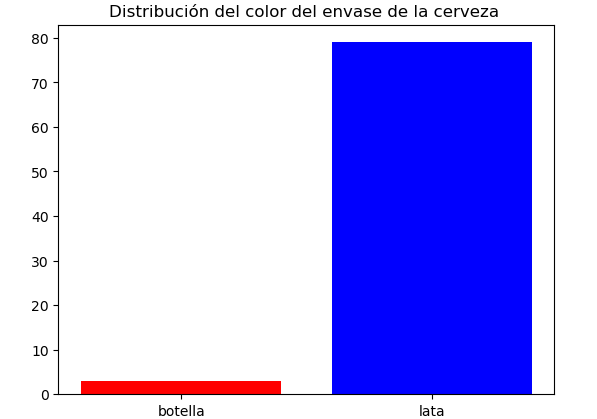
\includegraphics[scale=0.5]{envase cerveza.png}
    \end{frame}

\begin{frame}
    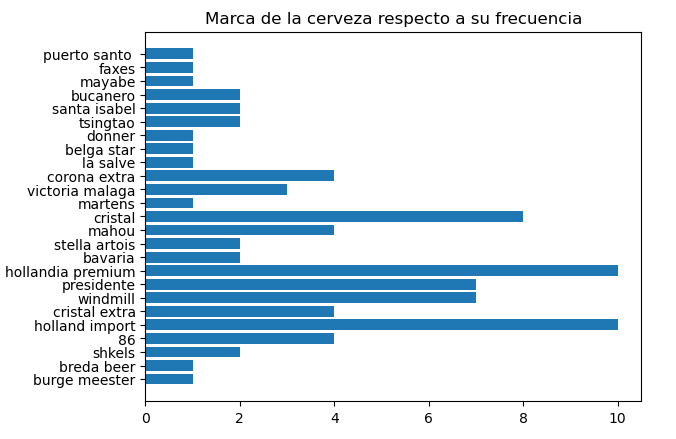
\includegraphics[scale=0.5]{marca de cerve.png}
    \end{frame}

\begin{frame}
    \includegraphics[scale=0.5]{volume cerveza.png}
    \end{frame}

\begin{frame}{Cebolla}
    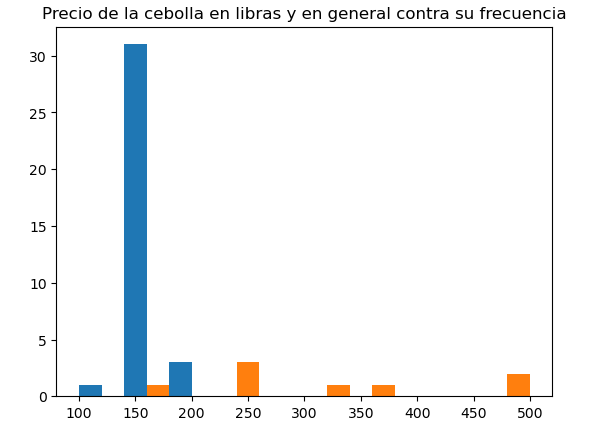
\includegraphics[scale=0.5]{precio de cebolla.png}
    \end{frame}

 \begin{frame}
    Aquí se aprecia la distribución del precio de la cebolla según el color
    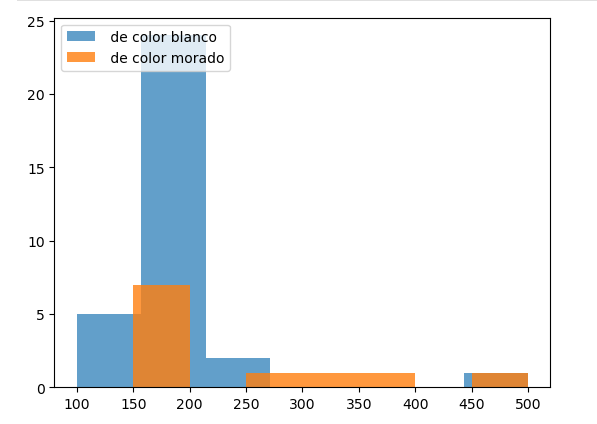
\includegraphics[scale=0.5]{precio por color cebolla.png}
    \end{frame}   

\begin{frame}
    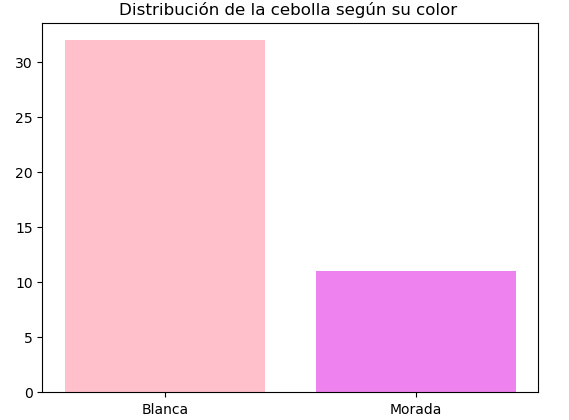
\includegraphics[scale=0.5]{color de la cebolla.png}
    \end{frame}
\begin{frame}{Comparación entre los refrescos envasados en botellas de plástico y en latas de aluminio.}
   \scriptsize 

    1-Los refrescos envasados en botellas de plástico:
    \footnote{\href{https://www.elfinanciero.com.mx/food-and-drink/2022/06/14/cual-sabe-mejor-refresco-en-vidrio-plastico-0-lata/?outputType=amp}{\textcolor{blue}{https://www.elfinanciero.com.mx/food-and-drink/2022/06/14/cual-sabe-mejor-refresco-en-vidrio-plastico-0-lata/?outputType=amp}}}
    \begin{itemize}
    
  \item Poseen acetaldehído que podrían pasar al refresco y afectar su sabor.
  \item El plástico es más permeable al CO2, la efervecencia de la bebida se escapa más rápido.
  \item Se derivan de productos no renovables.
  \item No se puede reciclar en más botellas.
  \item Las personas no reciclan botellas de plástico tan a menudo.
  \end{itemize}
  2-Los refrescos envasados en latas de aluminio:
  \footnote[2]{\href{https://medialab.news-latas-de-aluminoio-vs-botellas-de-plastico-cual-afecta-mas-al-medio-ambiente/?amp}{\textcolor{blue}{https://medialab.news-latas-de-aluminoio-vs-botellas-de-plastico-cual-afecta-mas-al-medio-ambiente/?amp}}}
  \begin{itemize}
  \item El interior de las latas está revestido con un polímero, que evita el contacto del refresco con el metal.
  \item Son menos permeables al CO2, conservan las burbujas por más tiempo.
  \item Proviene de la roca bausita, y su extracción puede arruinar ecosistemas.
  \item Se pueden reciclar en nuevas latas.
  \item Se estima que casi el 75 porciento de aluminio producido está en uso.
  \end{itemize}
  
Teniendo en cuenta las características de ambos envases, se analizarón los refrescos en latas de aluminio al poseer algunas ventajas.

  
\end{frame}

\begin{frame}
    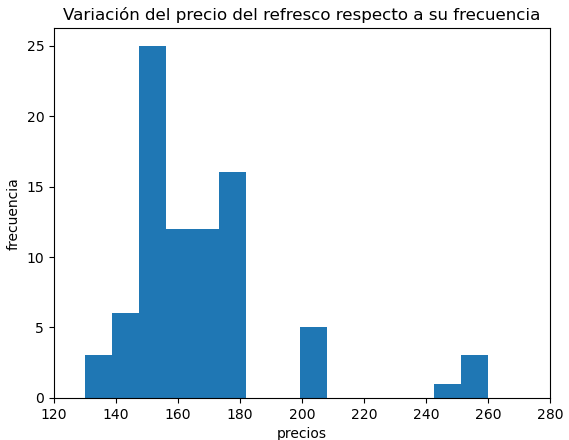
\includegraphics[scale=0.5]{precio de refresco.png}
    \end{frame}

\begin{frame}
    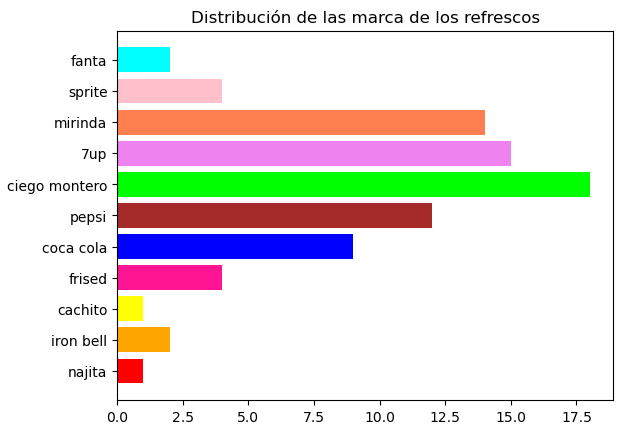
\includegraphics[scale=0.5]{marca de refresco.png}
    \end{frame}    

\begin{frame}
    Aquí se aprecia la relación marca y precio de los refrescos
    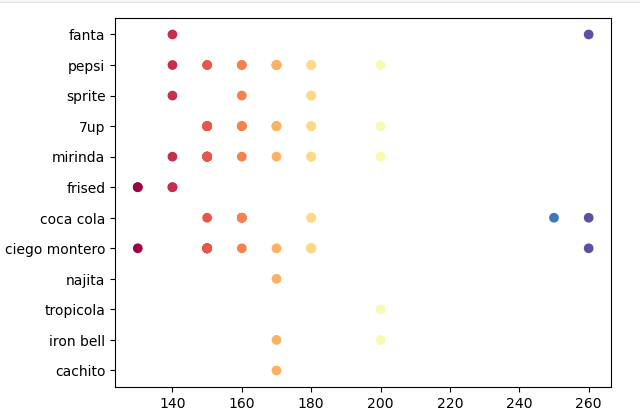
\includegraphics[scale=0.5]{marca y precio de refresco.png}
    \end{frame}    

\begin{frame}
    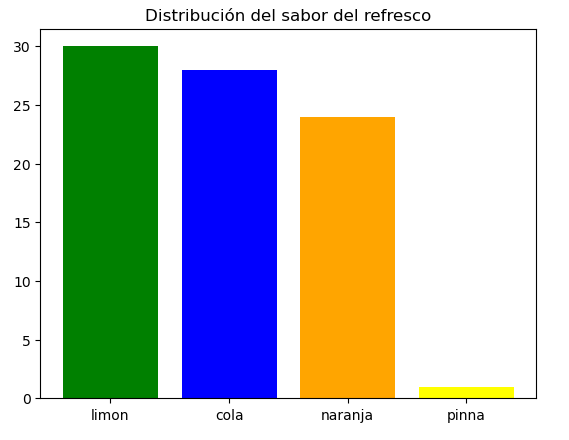
\includegraphics[scale=0.5]{sabor de refresco.png}
    \end{frame}

\begin{frame}
    En este mapa se aprecia la distribución de los refrescos(azul) y las cervezas(rojo)
    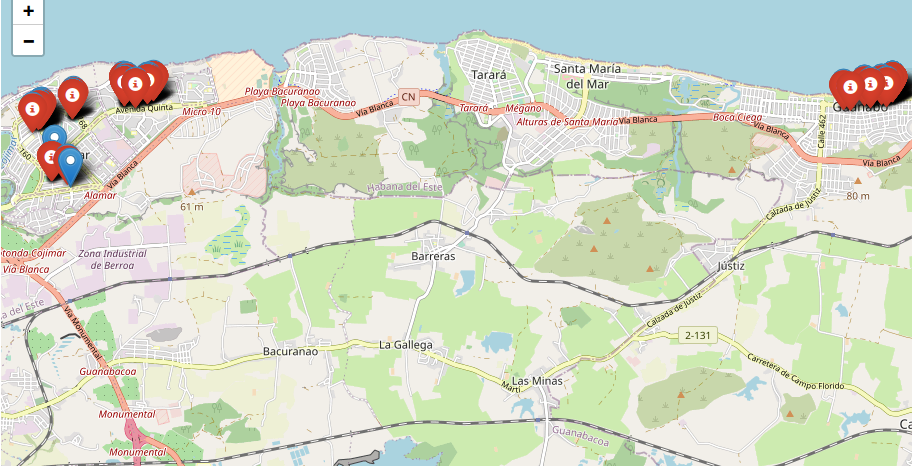
\includegraphics[scale=0.30]{mapa de cerveza y refresco.png}
    \end{frame}

\begin{frame}
    Aquí se aprecia la distribución de la cebolla según su color
    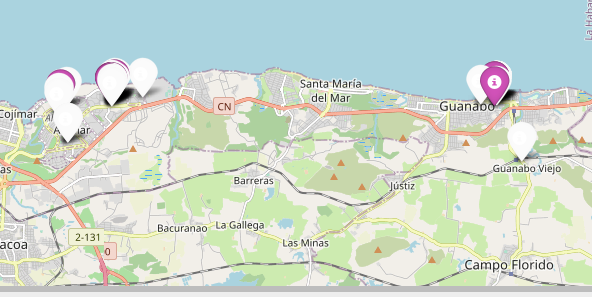
\includegraphics[scale=0.5]{mapa de cebolla.png}
    \end{frame}    
    
\end{document}